\newcommand{\NWtarget}[2]{#2}
\newcommand{\NWlink}[2]{#2}
\newcommand{\NWtxtMacroDefBy}{Fragment defined by}
\newcommand{\NWtxtMacroRefIn}{Fragment referenced in}
\newcommand{\NWtxtMacroNoRef}{Fragment never referenced}
\newcommand{\NWtxtDefBy}{Defined by}
\newcommand{\NWtxtRefIn}{Referenced in}
\newcommand{\NWtxtNoRef}{Not referenced}
\newcommand{\NWtxtFileDefBy}{File defined by}
\newcommand{\NWtxtIdentDefinedIn}{defined in}
\newcommand{\NWtxtIdentUsedIn}{used in}
\newcommand{\NWtxtIdentUsers}{Users:}
\newcommand{\NWtxtIdentsNotUsed}{never used}
\newcommand{\NWtxtIdentsUsed}{Uses:}
\newcommand{\NWsep}{${\diamond}$}
\newcommand{\NWnotglobal}{(not defined globally)}
\newcommand{\NWuseHyperlinks}{}
\documentclass[a4paper, 12pt]{article}
\usepackage{fullpage} % for 1.5 cm margins
\renewcommand{\familydefault}{\sfdefault} % so it doesn't look like LaTeX
\usepackage{helvet}
\usepackage{graphicx}
\graphicspath{ {imgs/} }
\usepackage{float} % so the figures stay with the text


\usepackage{abstract}
\renewcommand{\abstractname}{Overview}
\raggedright

\usepackage{parskip}

\usepackage[%
backref,%
raiselinks,%
pdfhighlight=/O,%
pagebackref,%
hyperfigures,%
breaklinks,%
colorlinks,%
pdfpagemode=None,%
pdfstartview=Fit,%
]{hyperref}

\title{Promethean Temperature Sensor}
\author{Joe J Collins}

\begin{document}
\maketitle
%%%%%%%%%%%%%%%%%%%%%%%%%%%%%%%%%%%%%%%%%%%%%%%%%%%%%%%%%%%%
\tableofcontents


%%%%%%%%%%%%%%%%%%%%%%%%%%%%%%%%%%%%%%%%%%%%%%%%%%%%%%%%%%%%
\section{The Problem}

Monitoring with Prometheus
no off the shelf monitoring.
Temperature is important.

\begin{description}
  \item[Start up time]
  \item[Maintenance]
  \item[Cost]
  \item[Availability]
  \item[Support information] 
\end{description}


%%%%%%%%%%%%%%%%%%%%%%%%%%%%%%%%%%%%%%%%%%%%%%%%%%%%%%%%%%%%
\section{Components}



\begin{figure}[H]
  \centering
  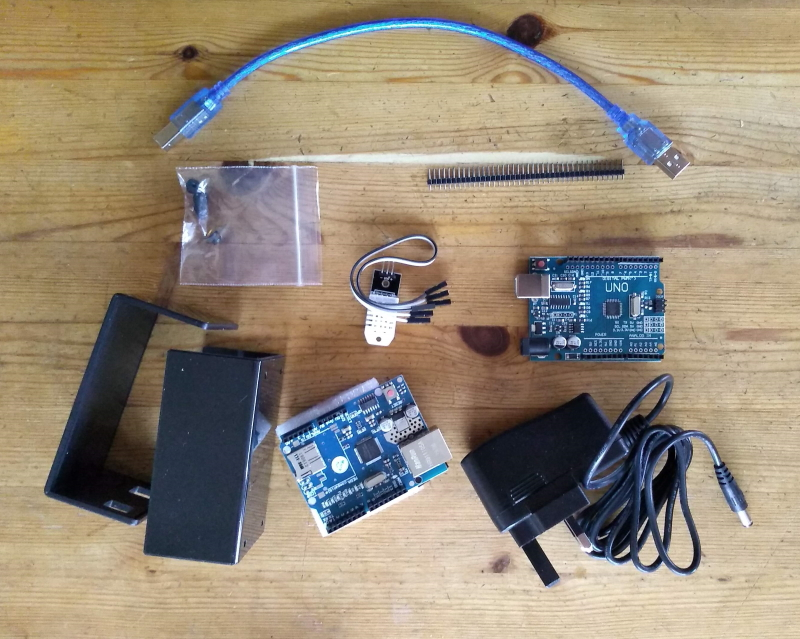
\includegraphics[width=0.8\textwidth]{components.jpg}
  \caption{Components}
\end{figure}

%%%%%%%%%%%%%%%%%%%%%%%%%%%%%%%%%%%%%%%%%%%%%%%%%%%%%%%%%%%%
\section{Wiring}

Pull up resistor.



\begin{figure}[H]
  \centering
  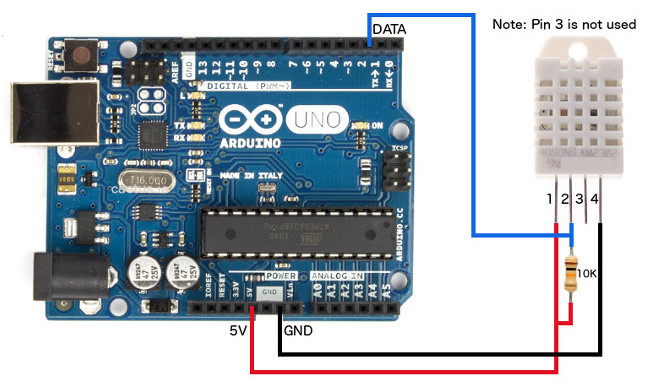
\includegraphics[width=0.8\textwidth]{wiring-dht22.jpg}
  \caption{Wiring diagram with pull up resistor}
\end{figure}



%%%%%%%%%%%%%%%%%%%%%%%%%%%%%%%%%%%%%%%%%%%%%%%%%%%%%%%%%%%%
\section{Programming}

Platform io

\begin{flushleft} \small
\begin{minipage}{\linewidth}\label{scrap1}\raggedright\small
\NWtarget{nuweb3a}{}\verb@"../src/shit.cpp"@\nobreak\ {\footnotesize{3a}}$\equiv$
\vspace{-1ex}
\begin{list}{}{\setlength{\leftmargin}{1em}} \item
\mbox{}\verb@#include <Arduino.h>@\\
\mbox{}\verb@@$\langle\,${\itshape libraries}\ {\footnotesize \NWlink{nuweb3b}{3b}}\,$\rangle\,$\verb@@\\
\mbox{}{\NWsep}
\end{list}
\vspace{-1ex}
\end{minipage}
\end{flushleft}


%%%%%%%%%%%%%%%%%%%%%%%%%%%%%%%%%%%%%%%%%%%%%%%%%%%%%%%%%%%%
\subsection{Libraries}

Notes

\begin{flushleft} \small
\begin{minipage}{\linewidth}\label{scrap2}\raggedright\small
\NWtarget{nuweb3b}{}$\langle\,${\itshape libraries}\nobreak\ {\footnotesize{3b}}$\,\rangle\equiv$
\vspace{-1ex}
\begin{list}{}{\setlength{\leftmargin}{1em}} \item
\mbox{}\verb@// Include the libraries:@\\
\mbox{}\verb@#include <Adafruit_Sensor.h>@\\
\mbox{}\verb@#include <DHT.h>@\\
\mbox{}\verb@#include <SPI.h>@\\
\mbox{}\verb@#include <Ethernet.h>@\\
\mbox{}{\NWsep}
\end{list}
\vspace{-1ex}
\vspace{-1ex}
\footnotesize
\begin{list}{}{\setlength{\itemsep}{-\parsep}\setlength{\itemindent}{-\leftmargin}}
\item \NWtxtMacroRefIn\ \NWlink{nuweb3a}{3a}.
\end{list}
\end{minipage}
\end{flushleft}


%%%%%%%%%%%%%%%%%%%%%%%%%%%%%%%%%%%%%%%%%%%%%%%%%%%%%%%%%%%%
\subsection{Upload}

Drivers on PC.



%%%%%%%%%%%%%%%%%%%%%%%%%%%%%%%%%%%%%%%%%%%%%%%%%%%%%%%%%%%%
\subsection{Testing}

\begin{verbatim}
  --- Quit: Ctrl+C | Menu: Ctrl+T | Help: Ctrl+T followed by Ctrl+H ---
  Webserver set up
  Sensor set up
  Humidity: 55.90 % | Temperature: 22.10 C
  Humidity: 56.30 % | Temperature: 22.20 C
  \end{verbatim}
  
  This is the endpoint at \url{http://192.168.1.2/}.
  
  \begin{verbatim}
  # HELP temperature is the last temperature reading in degrees celsius
  # TYPE temp gauge
  temperature 21.90
  # HELP humidity is the last relative humidity reading as a percentage
  # TYPE humidity gauge
  humidity 54.90
  \end{verbatim}

%%%%%%%%%%%%%%%%%%%%%%%%%%%%%%%%%%%%%%%%%%%%%%%%%%%%%%%%%%%%
\section{Packaging}

\begin{figure}[H]
  \centering
  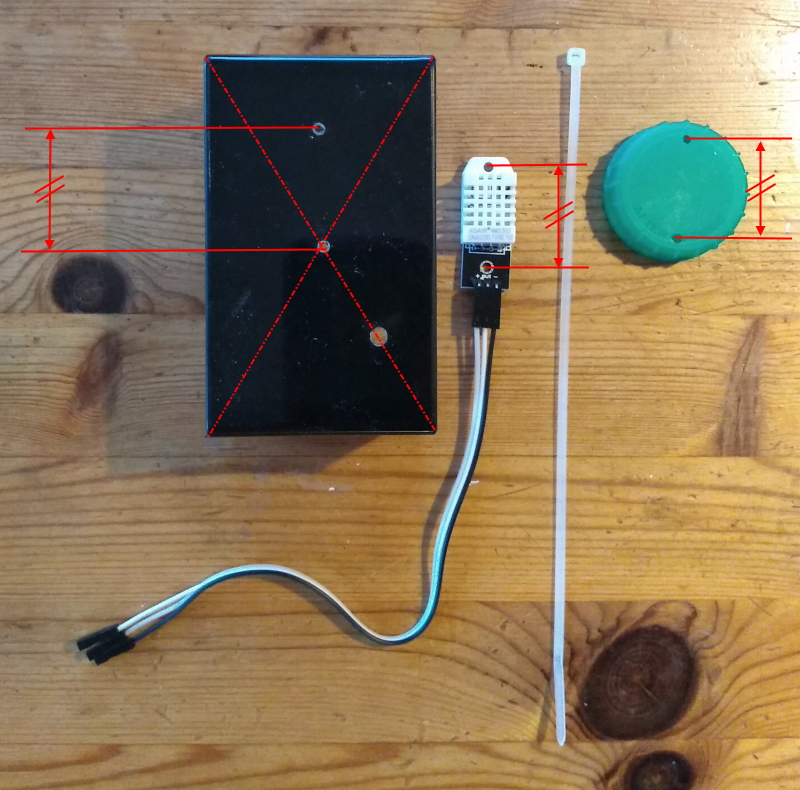
\includegraphics[width=0.8\textwidth]{sensor-mount.jpg}
  \caption{Components for mounting the sensor}
\end{figure}



2.5 mm holes and 4 mm holes.

\begin{figure}[H]
  \centering
  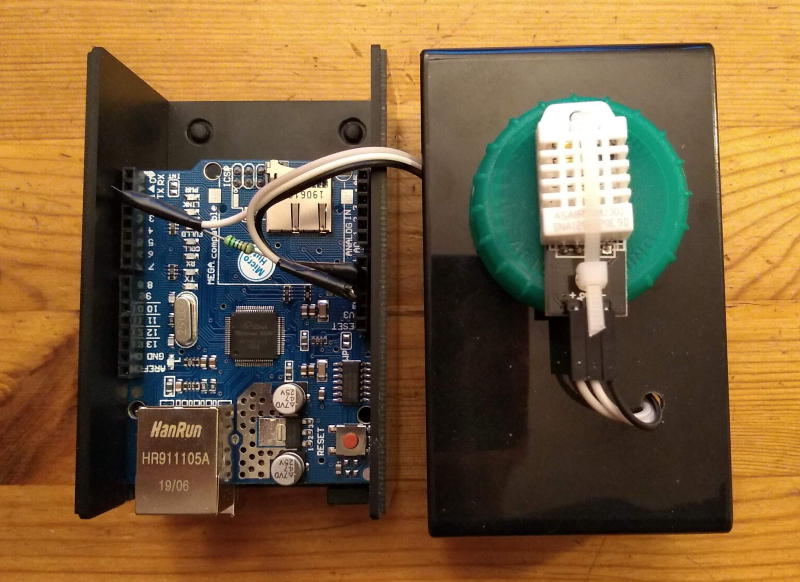
\includegraphics[width=0.8\textwidth]{packaging.jpg}
  \caption{Mounted sensor and wiring}
\end{figure}

\end{document}